% This is based on the LLNCS.DEM the demonstration file of
% the LaTeX macro package from Springer-Verlag
% for Lecture Notes in Computer Science,
% version 2.4 for LaTeX2e as of 16. April 2010
%
% See http://www.springer.com/computer/lncs/lncs+authors?SGWID=0-40209-0-0-0
% for the full guidelines.
%
\documentclass{llncs}
\usepackage{graphicx}
\usepackage[]{algorithm2e}

\begin{document}
\title{\LARGE \bf
Do you know what we are doing? Using human knowledge awareness on collaborative plan for relevant speech generation.
}
%
\titlerunning{HTN verbalization using agent belief awareness}  % abbreviated title (for running head)
%                                     also used for the TOC unless
%                                     \toctitle is used
%
\author{Gr\'egoire Milliez\inst{1} \and Rapha\"el Lallement\inst{1}
Michelangelo Fiore\inst{1} \and Rachid Alami\inst{1}}
%
\authorrunning{Gr\'egoire Milliez et al.} % abbreviated author list (for running head)
%
%%%% list of authors for the TOC (use if author list has to be modified)
\tocauthor{Gr\'egoire Milliez, Rapha\"el Lallement, Michelangelo Fiore, Rachid Alami}
%
\institute{Universit\'e de Toulouse, LAAS-CNRS institut Carnot,
        7 rue du Colonel Roche, 31500, France,\\
\email{firstname.surname@laas.fr},\\ home page:
\texttt{www.laas.fr}
}


\maketitle              % typeset the title of the contribution

\begin{abstract}
Robots are made to assist humans on daily basis tasks, either in households or at working places. In some situations, the task may require a collaborative plan computation and execution.
To achieve a collaborative plan, each agent need to be aware of their own task and how to perform them. This paper aims to address the issue of enhancing a robotic system with appropriate plan verbalization based on its dynamically updated collaborator's knowledge model.
 We will also explain how we can tune our shared plan generation to optimize it according to the user's knowledge level on each task, and how we use the tree configuration of our Hierarchical Task Network (HTN) plan to enhance the robotic system with an appropriate monitoring according to the partner's knowledge level on the current task.\dots
\keywords{HRI, HTN, perspective taking, speech generation}
\end{abstract}
%


%%%%%%%%%%%%%%%%%%%%%%%%%%%%%%%%%%%%%%%%%%%%%%%%%%%%%%%%%%%%%%%%%%%
% end abstract

\section{Introduction}
% Expose the issue of plan verbalizing + why HTN as colaborative plan + why reasoning on agent knowledge
One of the great challenges in robotics is to build a system able to collaborate with humans. Collaborating with human partners requires to plan for each agent, to monitor humans' inherently complex actions and dynamically update the environment model, but also to interact with the partner in a socially acceptable manner.
A collaborative plan, or shared plan, is a set of actions involving several agents that cooperate toward the same goal.
%Do we need that much of detail already? Or should we wait for part on HATP?
Some actions of the plan may be executed in parallel, sequentially or jointly (several agents acting together) and may require synchronization to ensure proper plan execution.
%

Once the robot has generated a collaborative plan to achieve the common goal, this plan needs to be shared with the human partners in order to insure that they are aware of the actions they have to perform and have the requested level of knowledge to perform their task. When dealing with simple plans, infants can cooperate without using language if the plan and goal are simple enough. In situations requiring more complex plans, language is the preferred method \cite{Warneken2006,Warneken2007}. However, we believe that just verbalizing the whole plan would be inefficient and 
annoying for the human partner, specially when he is already aware of the way to achieve part of it.  %%Miki: meta-tasks seems to be to specific at this level imo 


Research in psychology and philosophy lead to have a closer understanding on human behavior during joint actions and collaboration, to understand how \cite{tomasello2005} and why \cite{tomasello2009} we collaborate and what is shared during these interactions \cite{Butterfill2011}.

These research on joint actions were used in robotic platforms to perform tasks involving human partners. While many research deal with the issue of plan generation for collaborative goal implying a human partner,
since I do not want to go over your part :P%TODO RAPH: cite paper on collaborative plan generation
 few actually study how to share the plan in a socially acceptable way.
In this paper we will expose our way to solve this issue. We will first explain how we track human's knowledge, then how we are able to generate an HTN collaborative plan with a policy on human knowledge level on the actions in the plan. We will then explain how we use the tree structure of the HTN  plan generated to verbalize the shared plan according to the user knowledge level. To finish, we will expose how we use the HTN tree also during the execution phase to inform the human of the current execution step, to guide him while he performs new tasks and to have an adaptive monitoring of his actions. %% I think you can cut something here. Seems like we're applying the verbalization algorithm to our paper XD




%%%%%%%%%%%%%%%%%%%%%%%%%%%%%%%%%%%%%%%%%%%%%%%%%%%%%%%%%%%%%%%%%%
%end intro


\section{Related Works}

%%%%%%%%%%%%%%%%%%%%%%%%%%%%%%%%%%%%%%%%%%%%%%%%%%%%%%%%%%%%%%
%Plan verbalizing


%TODO: to use or not to use, that is the question...
%Successive Developmental Levels of Autobiographical Memory for Learning Through Social Interaction
%https://www.researchgate.net/publication/265555635_Successive_Developmental_Levels_of_Autobiographical_Memory_for_Learning_Through_Social_Interaction


%shrink?
\cite{Lallee2013} show that cooperation capability is significantly enhanced when the robot has a joint plan which allows it to guide the successive turn taking in achieving the execution. They also lead experiments on na\"ive subjects and suggest that the joint plan should be fully communicated in order to sustain effective collaboration. We argue that one way to improve the interaction with any kind of subject is by reasoning on human knowledge on tasks involved in the joint plan.

\cite{Brenner2008} presents Continual Collaborative Planning (CCP), a framework for behavior planning, physical action and perception. They show how mixed-initiative dialogue that interleaves physical  actions,  sensing,  and  communication  between
agents occurs naturally during CCP.

In \cite{Petit2012}, dialogue is used to teach new plans to the robot and to modify these plans. The authors presents three ways for the robot to learn: ``imitation'' where the human shows how to perform a task, ``kinesthetic teaching'' where the human manipulates the robot to teach a motion and ``spoken language programming'' where the human verbally explains the task to the robot. The robot is able to ask for the description of an unknown plan or action. However, in our situation the robot is the one that may have to explain the task and the use of HTN plans allows us to adapt the level of explanation to the knowledge level of the collaborator
%https://www.researchgate.net/publication/260662746_The_Coordinating_Role_of_Language_in_Real-Time_Multimodal_Learning_of_Cooperative_Tasks

%%%%%%%%%%%%%%%%%%%%%%%%%%%%%%%%%%%%%%%%%%%%%%%%%%%%%%%%%%%%%%
%use of perspective taking

% In psychology (2 / 3 papers)
%Define perspective taking

%Remove?
%In this paper, we choose to use the other agents' knowledge to adapt the plan verbalization.
Reasoning on others' mental state is a skill called Theory of Mind \cite{premack1978does}. An ability linked to this concept is perspective taking, which is widely studied in developmental literature. This broad term encompasses 1)
perceptual perspective taking, whereby 
humans can understand that other people see the world differently~\cite{Tversky1999}, and 2) 
conceptual perspective taking, whereby humans can go further and attribute thoughts and feelings to other people~\cite{Baron1985}.

%%%%%%%%%%%%%%%%%%%%%%%%%%%%%%%%%%%%%%%%%%%%%%%%%%%%%%%%%%%%%%%%%%%%%%%
% perspect t. in robotics

% In robotic, show how it is used to improve different things:
% planning, dialogue, intention recognition...
The perspective taking ability has been successfully used in several robotic fields, improving robots' reasoning capabilities, leading to more appropriate and efficient task planning and interaction strategies.
Among others, ~\cite{breazeal2006} presents a learning algorithm that takes into account information about a teacher's visual perspective in order to learn specific colored buttons activation/deactivation patterns.

Some studies also use conceptual perspective taking to manage agents' belief state and deal with divergent belief situations. Formulated in~\cite{wimmer1983}, this kind of task requires the ability to recognize that others can have beliefs about the world that differ from the observable reality.

In our previous work, we show how reasoning on others' mental state is a key feature for planning \cite{guitton2012}, understanding properly others' intentions \cite{fiore2015}, and improving dialogue \cite{Ferreira2015}. While these research focused on robot representation of other agents' belief state concerning the environment, here we will maintain and use a model of the human knowledge on the collaborative plan to perform as we believe that reasoning on partner mental state is a key feature during joint action.


%TODO: where to put this?
%Theory of mind and dialogic act
%This  paper  has  attempted  to  show  that  we  can  define  communicative  acts  in  terms  of  the  mental  states  of  the  agents  performing  the  act,  and  that  these  acts  are  effective  ways  to  form,  regulate  and  disband  teams  of  agents.  The  mental  states  of  the  agents  include  the  commitments  the  agents  in  a  team  have  toward  each  other  and  toward  the  team ’ s  task.  These  communications  acts  and  the  mental  states  they  represent  can  be  used  as  the  basis  for  an  agent  communication  language ’ s  semantics.  We  have  applied  the  theory  to  a  model  of  interagent  protocol,  and  shown  the  theory  explains  the  structure  of  that  protocol.  In  the  process  we  have  demonstrated  that  our  small  set  of  primitive  acts  can  be  composed  to  define  more  complex  communicative  acts.  Our  policy  of  building  new  operators  from  an  existing  set  of  well-defined  primitives  leads  to  a  consistent  and  well-understood  semantics  for  the  language.  Furthermore,  it  offers  the  possibility  that  agents  can  themselves  enlarge  the  set  of  communicative  actions  by  decomposing  non-primitive  ones  into  their  more  primitive  parts. 
%https://www.aaai.org/Papers/AAAI/1996/AAAI96-004.pdf


%%%%%%%%%%%%%%%%%%%%%%%%%%%%%%%%%%%%%%%%%%%%%%%%%%%%%%%%%
%Planning


% Why use of HTN for adaptive verbalization level?
% papers on learning amount policy?
%TODO Raph

%%Miki:Is this really related works? Shouldn't it go later? If not shouldn't we fuse introduction and related works together?
We chose to use HTN structures to represent shared plans because it's a hierarchical composition. Planners such as STRIPS \cite{strips71} build plans that are simply sequences of actions. On the other hand hierarchy offers a better understanding of the context in which an agent is asked to carry out an action. This context can be used by the monitoring system to better track the execution of the action but it is also very beneficial for dialogue. Indeed, by understanding the reasons behind an action, the dialogue system guide users in a more appropriate way, by explaining why he should perform an action and how it is linked to previous and successive part of the plan. 


There are several types of hierarchical planners. We are using the widespread HTN because its domain representation and its algorithm are easy to understand, which makes it a good robotics tool, while still being very efficient. It is way more efficient than classical planning since the domain expert can guide the search process toward the goal by providing a correct representation. 

A very famous implementation of HTN is SHOP \cite{Nau99}. Our planner will be described in section \ref{planning}.


%%%%%%%%%%%%%%%%%%%%%%%%%%%%%%%%%%%%%%%%%%%%%%%%%%%%%%%%%%%%
%%Plan Monitoring
Concerning monitoring, to keep track on the plan's status we must first understand what each participant is doing. There are several approaches to action recognition in research. One inspired by psychology, aim at recognizing actions by simulating behaviors in the robot schemes \cite{gray2005action} \cite{demiris2006hierarchical}.

%Action recognition has been studied in research, based on different approach. For example, in \cite{gray2005action} the robot monitors users' actions by simulating their behaviors with the robot's motor, goal and perceptual levels. In \cite{demiris2006hierarchical} the authors present the HAMMER
%architecture, based on the idea of using inverse and forward models
%arranged in hierarchical and parallel manners. With this architecture
%the authors are able to use the same model to execute and recognize
%actions, an idea compatible with several biological evidences. 

Other psychological studies show that when performing joint actions, humans use several skills, and form a shared representation of the task, which includes the actions that every partner should perform \cite{sebanz2006joint}. The monitored actions must, then, be linked to this shared representation of the task in order to understand the engagement level of each member of the joint action, and if there are errors that need to be repaired. 

\cite{nikolaidis2013human} applies cross-training  to shared-planning. A human and a robot iteratively switch roles to learn a shared plan for a collaborative task. This strategy is compared to standard reinforcement learning techniques, showing improvements in performances. These results support the idea of modeling practices for human teamwork in human robot interaction.

Some systems explicitly model shared plans during task execution, allowing robot to adapt their plans to the users' actions, like Pike \cite{levine2014concurrent,karpas2015robust}, and Chaski \cite{shah2011improved}.


In \cite{clairrobot} dialogue is used during collaborative plan execution in order to improve the performances of the team. The paper uses an approach based on Markov Decision Problems and gives importance on the concept of agent roles in a task, which can be estimated and influenced using dialogue. 


%\cite{levine2014concurrent} shows Pike, a system able to form a shared plan,  recognize human plans and adapt the robot's actions. Pike was further improved in \cite{karpas2015robust}, adding robustness to temporal uncertainty in action execution.

%TODO Michelangelo:
% Add this paper?
%http://robotics.usc.edu/publications/media/uploads/pubs/hrifp2561-st-clair.pdf




%In \cite{shah2011improved} a shared plan is executed
%using Chaski, a task-level executive which is used to adapt the robot's actions to the human partners. Plans can be executed in two different modalities: equal partners or leader and assistant. 




%%%%%%%%%%%%%%%%%%%%%%%%%%%%%%%%%%%%%%%%%%%%%%%%%%%%%%%%%%%%%%%%%
%end related works






\section{Knowledge Tracking}
Reasoning on agents' knowledge requires first that the robot manage a mental state for each agent involved in the interaction.

In this context, as the robot will generate the shared plan, we will suppose that it knows all the actions included in the plan.

% => Greg
% (toaster)
\subsection{Situation Assessment}
To assess the mental state of its collaborator, the robot needs to understand the situation and extract information about agents' beliefs and knowledge.
To do so, we use the toaster framework (Tracking Of Agents and Spatio-TEmporal Reasoning). Toaster is a modular framework meant to fill the gap between perception and decision layers. It uses data about humans, robots and objects to asses the situation and to maintain a consistent world state. It also computes affordances for each agent (reachability and visibility).

We won't detail here any further this component concerning the situation assessment.
For more details see our previous work with SPARK \cite{Milliez2014}.

\subsection{Mental States}
% present our way of maintaining belief state
Using situation assessment, we were able in previous works to manage a belief state for each agent, robots and humans. Each belief state model is independent and logically consistent. The models represent the way the robot represent its counterparts' mental states about the environment.

In this paper we won't consider beliefs on environment but only consider the human's knowledge on actions. This knowledge will be represented as a set of 4 variables, consisting in the human agent it is linked to, the kind of action, a list of parameter and the value (or level) of knowledge:

AGENT ACTION PARAMETERS VALUE

As an example, the fact that the human (\textit{human1}) has a "practical" knowledge on cooking an apple-pie would be represented as:

human1 cook applePie practical

The different possible values are \textit{unknown}, \textit{theoretical} and \textit{practical}. More details on these values will be given in the next part.

For some actions, the knowledge may be linked to a "class" of parameters while in others it will be related to an instance of this class.
Let's consider a scenario where two agents have to process colored cubes and stack them.
The action \textit{process} may differ depending on which cube we are processing: we may want to paint the red cube and to polish the green cube. %Miki: sounded a little bad before I think

In this case we will represent this knowledge as follow:

AGENT process greenCube VALUE

For other actions, the knowledge will be specific to a class. As an example if a human knows how to polish the green cube, we consider that he will know how to polish any cube.

%Miki:imo the example is not very clear. I think you should specify the relation between process and polish (i.e. polish is a sub-task in process or a decomposition if a i got it right)
% GREG: there are no relations between the two. I will change the examples...

In that case, we will represent this knowledge as follow:

AGENT polish cubes VALUE

%TODO RAPH:
%check if we can do this in a better way
In the current implementation, the fact that an action is specific to an instance of the parameter or generalized to a class of parameter is hard-coded and planification domain dependent.

%comment RAPH: This is related to the fact that we want to make it automatic but did not spent time on it ... should we  work on it ?
%comment RAPH: Otherwise what do you expect from me in this section ? Because in the end HATP is using the knowledge only to compute the cost ... I started to write about it but if you feel it misses some details we should decide what to add since I do not want to go over your part :P

%comment GREG: Couldn't there be a tag, to tell this action is linked to a class of parameter and maybe what class?
\subsection{Updating Knowledge}

%How human update their knowledge
There are several ways for humans to modify their state of knowledge. To track human mental state we need to identify these ways.

%1) Someone explain
\subsubsection{Getting information from a third party}
The first way for a human to acquire knowledge is to get explanations from a third party. In our system, when a human is informed of how to perform an action, we will change the value of his knowledge from \textit{unknown} to \textit{theoretical} to represent that he has been told of what to do when we ask him to perform this task.

%2) Someone did task in front of agent
\subsubsection{Observation and analyze}
% Human can learn to do something by seeing somebody else doing it.
%
%TODO: check redondant with Michelangelo on role reversal
Another way for humans to learn is through observation and imitation of a third party achieving the action. Studies in developmental psychology show evidence that role reversal imitation ability is present in developing infants \cite{carpenter2005}.
In our system, when a human will observe someone else perform an action, we will set his knowledge value of this action from \textit{theoretical} to \textit{practical}. In this setting we will consider that, if a human observes an action being performed without actually being instructed of the action, he won't be able to link it to the corresponding action. So if a human with a knowledge value set to \textit{unknown} observes this action being performed, we won't update his knowledge value and consider that he still needs explanation.
%The current research thus exploits a series of developments that have resulted in the ability of the robot to learn a joint plan, to use that joint plan in cooperation with a human, and to demonstrate role reversal  [6-8].  Again, in role reversal, the cognitive agent is able to use the same joint plan, but exchange roles with the other partner.  This ability has been recognized by developmental psychologists as evidence that the agent has “bird’s eye view” knowledge of the joint plan, rather than a purely ego-centric view  [17].

%https://www.researchgate.net/publication/260662746_The_Coordinating_Role_of_Language_in_Real-Time_Multimodal_Learning_of_Cooperative_Tasks

%In role reversal, the cognitive agent is able to use the same joint plan, but exchange roles with the other partner. This ability has been recognized by developmental psychologists as evidence that the agent has “bird’s eye view” knowledge of the joint plan, rather than a purely ego-centric view  [17].

%M. Carpenter, M. Tomasello, and T. Striano, ``Role reversal imitation and language in typically developing infants and children with autism,'' Infancy, vol. 8, pp. 253-278, 2005.



%3) Agent did the task

%The observations made possible via both exploratory and performatory actions  provide the material for his knowledge of the world
%http://wexler.free.fr/library/files/gibson%20%281988%29%20exploratory%20behavior%20in%20the%20development%20of%20perceiving,%20acting,%20and%20the%20acquiring%20of%20knowledge.pdf

\subsubsection{Task performed}
The last knowledge state transition we will consider is when the human actually succeeds to perform the task. When a human performs a new task, we will change his knowledge state from to \textit{practical}.


%4) Agent failed to do the task
% TODO: verify that the supervisor can get the failures
\subsubsection{Task failure}
It may happen during the execution that a human fails to perform a task.
We will then reduce his knowledge on this task to \textit{theoretical} if it's the first failure and to \textit{unknown} if he fails several times to achieve the action.

%5) Agent require explanation
\subsubsection{Information request}
It may happen during the execution that a human directly asks for information on a task.
If the human asks what to do, we will lower his task knowledge level to \textit{unknown}. If he asks how to do the task, we will only lower his task knowledge level to \textit{theoretical}.

These different levels of knowledge will be used during the two verbalization steps. If an action is unknown to a human, we will explain it to him before starting the execution. If he has only theoretical knowledge of the action, we will explain him again during the execution and monitor each step of this action execution. More details will be given in \ref{planVerbalization} and \ref{execution}

%%%%%%%%%%%%%%%%%%%%%%%%%%%%%%%%%%%%%%%%%%%%%%%%%%%%%%%%%
% end knowledge


\section{Knowledge Level Policy For HTN Generation}
\label{planning}
% => TODO RAPH
%HATP
To compute collaborative plans, we use HATP \cite{lallement14} an HTN planner specifically designed for robotics. 
%TODO mb: some features related to plan generation such as...
HATP comes along with specific features such as: (1) agent based to allow multi-agent plans, (2) cost driven to allow plan pruning and (3) social rules to refine plan according to the most suited social behavior.

HATP multi-agent capabilities create plans with several streams, one per agent. The stream-plan produced can have parallel actions, or sequential actions, or joint actions so it can adapt to many situations. Since it is cost-driven the number of plan to compute is reduced: when computing all the plan to find the very best plan (in term of cost and properties it holds) if the current best plan is better than the current plan (even if incomplete) then the current plan is discarded and a new plan is tried. This mechanism reduces the number of plans to compute to obtain the best plan. This best plan is defined by its cost (the sum of every action's cost in the plan) but also by a set of social properties. Among others, some of those properties can be how the workload is shared, how often the human has to wait for the robot, the presence of undesired states.

To take knowledge in account while planning a new social rule was needed. The aim is to filter plans out if they do not match our knowledge policy. We propose two different policies: favor teaching so the human can learn from the robot or prefer efficiency. In the first case the planner tries to produce plans maximizing the number of human actions where the human must learn, while the second policy makes the planner 
%TODO: compute or chose?
compute plans with the least amount of unknown actions for the human in order to ensure that he can be more efficient (the robot however can execute some actions unknown to the human).

%TODO, make it more clear!
% mb just explain 1 policy is enough, and say we proceed in a similar way for the opposite?
%+ replace learning by teaching!
The principle of the rule is simply to apply a penalty every time the human has to perform an action he already knows (resp. he has to learn) so the solution plan chosen among all possible plan will contains the minimum number of known actions (resp. actions to learn) hence be more in favor of learning (resp. efficiency). The responsibility to decide between favoring learning or efficiency is then left to the domain expert (e.g. the company owner).

To illustrate this mechanism we can imagine a toy example where we want to clean a cube. There are two ways of doing it: using a rag or using water. We have two agents, a human and a robot, and they are both able to perform each step. However the human only knows how to clean with water. If we favor teaching then HATP will choose a plan where the human has to clean the cube using the rag (the robot will assist by providing dialogue guidance). On the other hand if we prefer efficiency there are two solutions : either the robot does the operation or the human uses water to clean the cube. 
%comment: je trouve que cette dernière phrase embrouille plus qu'autre chose soit reformuler, soit enlever
To choose between those last possibilities only the relative cost (e.g. of the motions) will determine which will be the solution used.


%%%%%%%%%%%%%%%%%%%%%%%%%%%%%%%%%%%%%%%%%%%%%%%%%%%%%%%%%%%
% end HTN

\section{Dynamically Adaptive Plan Verbalization}
\label{planVerbalization}
%htn_verbalizer => Greg

% intro
Once the robotic system has generated a collaborative plan adapted to the chosen HATP policy, the plan must be shared with the human partners.
Speech is a ``potent modality for the on-going maintenance of cooperative interaction'' \cite{Lallee2013}. Indeed, Tomasello even suggest that the principal function of language is to establish and negotiate cooperative plans \cite{tomasello2005}.
Considering this, we decide to use speech to verbalize the shared plan. We propose here a way to take advantage of the HTN collaborative plan structure to enhance an efficient plan verbalization.

Note: our verbalization module is able to look at object or agents during speech to give social cues and reinforce the communication, however as the multimodality is not the focus of our paper we won't give details on this aspect. Moreover, as this paper focus on efficient and socially acceptable way to verbalize a plan, we won't discuss the issue of negotiating a plan between the involved collaborators. The human will have to "accept" the plan generated by the robot.

The plan verbalization will occur in two steps.
During the first step, the robot will present the plan to the collaborators to inform them of "what" each agent should do, while in a second step, the robot will verbalize the actions to perform during the execution to guide its partners when they learn a new task or to inform them of the current state in order to reduce collisions and error rate during the execution.


%TODO:
%explain 1st step and tell that 2cd step will be explained in next part
\subsection{Plan preprocessing}
\label{preprocess}
When verbalizing the plan, we need to preprocess the node list we have from the plan tree to generate a verbalization tree.
During this operation we apply two rules.

The first rule is to replace the recursive actions by their children as we believe that recursive actions are useful for planning but confusing during plan explanation. To do so, we check if the parent node has the same action name and parameters then the children and if so, we remove the current node in the verbalizing list and replace it by its children.

%TODO: put an illustration here
\begin{figure}[ht!]
 \centering
 \begin{tabular}{cc}
  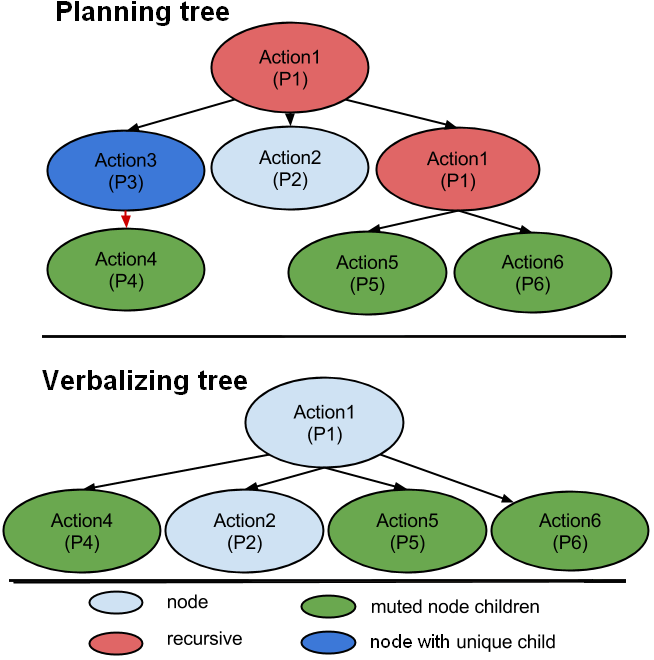
\includegraphics[width=0.9\textwidth]{img/rules.png}
 \end{tabular}
 \caption{HTN tree before and after speech processing. We don't verbalize recursive task (action1) and the one with unique child (action3).}
 \label{fig:tree_processing}
   \vspace{-6pt}
 \end{figure}
Second rule consist in reducing the verbalization tree by using child of an action instead of the action, if the child is unique.

These two rules are represented in the figure \ref{fig:tree_processing}, Action2 has a unique child. In the node list to verbalize, we will therefore replace it by its child. Action1 has the same name and parameter as it's parent. It means it's a recursive action so we won't verbalize it and we will replace it by its children in the node list to verbalize.

This processing is done during the verbalization, as shown in \ref{verbalizeNodes} function (processNodes function).


\subsection{Verbalization}

When a request is sent to the verbalization module to verbalize a tree, may it be the full plan or a sub-tree of the plan, we will call a first function to verbalize the root of this tree. As the root is the meta-task, we consider it as the goal and we will verbalize it regardless of the knowledge level of the agents.

So the verbalization of the tree will always start with an explanation of the goal.
The output sentence will look like this:
Pronoun + ``have to'' + task explanation.
The pronoun is determined according to the agents concerned. It can get the value ``I'', ``you'', ``we'' or even directly the name of agent in case of multiparty interaction.

Once this verbalization is done, we will look at the knowledge level of this root action to decide either to verbalize children or not.

%remove?
%, as shown in \ref{VerbalizeTree}.

%Do we really need this algo?
%\begin{algorithm}[H]
%\KwData{root node $r$}
%$tellGoal(involvedAgents, planToSpeech(r))$\;
%	\If{$getKnowledge(r) == "unknown"$} {
%        $verbalizeNodes(children(r))$\;
%}

%\caption{$verbalize\_tree$ \label{VerbalizeTree}}

%\end{algorithm}

In case the plan needs to be verbalized (the knowledge level of involved humans was not enough), we will verbalize the processed list of his children as explained in \ref{preprocess}.
To have a link between actions, we will verbalize differently according to the node position in the list.
For the first node, we will begin with: \textit{``To '' + planToSpeech(dad) + ``we will first'' + planToSpeech(currentNode)}. For the second node we will start the sentence with ``then'', and with ``finally'' for the last node.
%Miki: wouldn't it be better to add some randomness to the word to make it more variable?
%TODO: find a better example?
As an example, if a human is not aware on how to process the green cube, the system will verbalize its children as follow:
"To process the green cube, you will first pick it, then you will place it on the polishing area. Finally you will polish it". 

This proceeding is a depth-first research of nodes to verbalize. We believe this mode facilitates understanding as we will explain from meta-tasks to lower level. However the verbalization itself is not depth-first as it is done on every siblings of the current node before going deeper in the tree. While going into detail, the user still have an understanding on the task context.
To do so, after each node verbalization, we verify the knowledge level of the current node, and if the level is too low, we will add the children
%COMMENT: DO WE NEED TO EXPLAIN fifO?
to a FIFO queue to verbalize them after the current list siblings has been verbalized as shown in \ref{verbalizeNodes}. 
This implies that if the current node is a leaf, the level of knowledge on this action won't have any effect as this node has no children. This means that human needs to have knowledge on the atomic actions of the HTN.
%TODO should we really say that?
We believe that this is indeed usually the case.

One interesting aspect here is the dynamic update of the knowledge database.
If the knowledge level of an action is unknown, after all his children nodes have been verbalized, we will set the knowledge in database from \textit{unknown} to \textit{theoretical}.

Consequently, if an action has to be performed twice, we will explain it only once as at the second occurrence the knowledge level of the agent will be \textit{theoretical}.

\begin{algorithm}[H]
\KwData{parent node $dad$, children $list<node>$ $children$}
$processedChildren = processNodes(dad, children)$\;
\For{$n\leftarrow 0$ \KwTo $prossessedChildren(r)$}{
    $verbalizeList\leftarrow n$\;
	\If{$agents(n)!=robot AND getKnowledge(n) == "unknown"$} {
        $add\_queue{children(n), n}$\;
    }
}
\If{$getKnowledge(dad) == "unknown"$}{
	$setKnowledge(dad, getAgents(dad), "instructed")$\;
}
\While{$queue != \emptyset$}{
	$verbalize\_nodes{getFirstChildren(queue), getFirstDad(queue)}$\;
    $pop\_front(queue)$\;
}

    \caption{$verbalize\_nodes$ \label{verbalizeNodes}}

\end{algorithm}

This plan verbalization allow the user to have a global view of the plan and a first explanation of the task to perform with the order.

However, even if we believe this step is needed, we also think that it's not enough and a verbalization during execution is also needed to inform the user of the plan state, to avoid collisions and enhance task parallelization. This step will be explained in the following section.
% method




%
%%%%%%%%%%%%%%%%%%%%%%%%%%%%%%%%%%%%%%%%%%%%%%%%%%%%%%%%%%%%%%%%%%%%
% end verbalization

%GREG PROPOSITION

\section{Execution and Monitoring}
\label{execution1}

When the plan has been verbalized to give a global picture and to instruct the human partner of the new tasks in this plan the system will start executing the shared plan, interacting and monitoring the human partner in the process.

\subsection{Verbalization and Monitoring}
During execution,  the robot will signal using speech the start and the end of an action. As for the previous step, the level of refinement in the verbalization will depend on the knowledge level of the human partner.

%%Miki: I think this is irrelevant since we are executing the tree, that of course is execute depth first, and verbalization is linked to execution.
%The main difference is that we will verbalize here using depth-first. This means that if the human hasn't enough knowledge on a meta action, we will explain it before explaining its siblings.

%We decide to use this different policy as the human already has a global idea of the plan, and during the execution we want him to focus on the current task.
Once the current task to perform has been verbalized, the robot will perform it if he is the actor, or he will activate the monitoring on this action if the human is the actor. This means that the monitoring may be done on high-level tasks if the human has enough knowledge on the task.
%%Miki: changed a little here. Thoughts?
We chose this adaptive way of monitoring as we believe the robot would be more efficient, sparing his resources, by focusing its attention more often on parts of the plan that have never been performed by the human partner, and less when he has some form of expertise.
To explain this further, an example will be exposed in \ref{results}.

Monitoring human actions is complex, particularly in high-level tasks, were we are not monitoring a set of atomic actions. The system should have reasoning models that allow the robot to understand if the state of the world is coherent with the action that the human need to perform. The system should also be able to measure the level of engagement in the task of the human agent, to understand when the human is not executing his part of the shared plan, and react accordingly.

We choose for this first implementation a simple strategy for monitoring. The robot will observe the environment, updating its world state accordingly, and monitor the expected consequences of actions. We will consider an action as "failed" if it hasn't been performed before a predefined amount of time. We plan to extend this approach in the future, providing better mechanisms to measure the engagement of a human in a task and to understand when a monitored task has failed.


\subsection{Failure and replanning}

The goal of monitoring human actions is to be able to recover from unexpected behaviors of the human. When this happens, the robot will inform the human of his wrong behavior and decrease his knowledge on the current action to "theoretical". 
%maybe also the dad function to unknown to regive the context?
The robot will also ask the task planner to compute a new plan to achieve the goal with the current updated world state.
One of the benefit of the dynamical update of human knowledge is that this new plan may have meta-tasks that the robot already explained or that the human even performed before the failed action. In this case, informing the human of the new plan will be faster and we won't have to reexplain tasks that he already performed.

This replanning behavior give robustness to the robotic system and allow a socially acceptable recovery procedure where we inform the human error and reexplain the plan only on needed level of detail, as we took into account his knowledge improvement during the execution that failed.


%%Miki: Everything down seems to be irrelevant after this section so I commented it.
% %%%%%%%%%%%%%%%%%%%%%%%%%%%%%%%%%%%%%%%%%%%%%%%%%%%%%%%%
% \section{Execution and Monitoring}
% \label{execution}
% % => Michelangelo supervisor
% % + Greg
% Our approach enhances our previous work \cite{fioreiser2014} in which we propose a human-robot architecture with a supervision system able to execute in a flexible way plans involving a human partner.

% % The supervision system is built with the goal of being flexible and easily extended, creating new domains with different situations, environments and possible actions. The supervision system can also interact with different planners and robot platforms. In this section we will explain the aspects of the system that are more relevant to the paper.

% \subsection{Plan Management}
% When the supervision system receives a goal, which can be chosen by the robot based on the current domain and on the status or the robot or received from a user, the supervision system will require a shared plan to HATP.
% %composed by the actions of each participants. 

% This plan needs to be analyzed in order to discover two information: which tasks need to be verbalized by the robot during the execution and which user actions need to be monitored.  

%harmonize this as well. Is it needed? put it only once?
%+ use same convention
%I think we can just say that we use the same idea as before, except that this time we will use depth-first both for research of nodes to verbalize and for the verbalization itself. Meaning that we verbalize children before siblings. And same for monitoring.


%Old verion:

%The following algorithm shows how this analysis is performed.

%We define the following properties for the nodes $n$ in the tree $T$ and to the agents $a$:
%\begin{itemize}
%\item $recursive(n)$: the node represents is a recursive method from the HTN domain.
%\item $children(n)$: the list of children of $n$.
%\item $father(n)$: the father of $n$.
%\item $agents(n)$: the list of agents that participate in the task linked to $n$.
%\item $K(a,n)$: coefficient of knowledge of agent $a$ for the task associated to node $n$.
%\end{itemize}



%\begin{algorithm}[H]
%\KwData{root node $r$}
%	\If{$agents(r)==robot$} {
%        $verbalizeList\leftarrow nr$\;
%    	$analyzeChildren\leftarrow false$\;
%    }
%    \ElseIf{$robot \in agents(r)$} {
%        $verbalizeList\leftarrow r$\;
%        $analyzeChildren\leftarrow true$\;
%    }
%    \ElseIf{$(\exists a\in agents(r) | K(a)<C)$}  {
%        $verbalizeList\leftarrow r$\;
%        $analyzeChildren\leftarrow true$\;
 %   }
  %  \Else{
   % 	$verbalizeList\leftarrow r$\,
 %		$monitorList\leftarrow r$\,
 %		$analyzeChildren\leftarrow true$\;
  %  }

	%\If{analyzeChildren==true} {
	%	\For{$n\leftarrow 0$ \KwTo $children(r)$}{
	%		$analyze_tree(n)$
	%	}
  %
	%}

    %\caption{$analyze\_tree$ \label{AnalyzeTree}}

%\end{algorithm}

%TODO: no more threshold. monitor = other value than practical
%The idea of the algorithm is to verbalize only high-level tasks performed by the robot and to have a more complex verbalization and monitoring reasoning for humans. In general, we want to verbalize human actions when the agent has a coefficient of knowledge related to the task lower than a prefixed value. We will monitor the last highest human node in a sub-tree where the human has a knowledge value on the task higher than a threshold.
%%%%

%END OLD VERSION

% This process is similar to the plan verbalization algorithm, with some differences. The system will verbalize only high-level tasks performed by the robot and have a more adaptive process for the human actions' verbalization depending on his knowledge.
% The algorithm must also link each verbalization utterance with the corresponding action to perform or monitor. The robot will speak before and at the end of the execution of an action, in order to inform the human partner of the status of the task.  


% \subsection{Environment Monitoring}
% The supervision system will always keep track of the world status.
% Actions are represented in the supervision system as a tuple [preconditions, trigger, postconditions]. The preconditions are the facts that must be true in order to perform the action, the trigger is an object associated to the action, and the postconditions are the facts that will be true after performing the action.

% Using preconditions, the system is able to understand what actions can be performed by agents at a given moment.

% To understand when an action has been performed we use geometrical computation based on the human arm position related to points of interest in the environment. 
% % understand or estimate?
% In this way we can understand when a human executes an action and update the world status using the postconditions associated to the action.

% \subsection{Plan Monitoring \label{planMonitor}}
% Monitoring human actions is complex, particularly in high-level tasks, were we are not monitoring a set of atomic actions. The system should have reasoning models that allow the robot to understand if the state of the world is coherent with the action that the human need to perform. The system should also be able to measure the level of engagement in the task of the human agent, to understand when the human is not executing his part of the shared plan, and react accordingly.

% %comment: I modified, verify it
% % TODO: speak about knowledge update
% In our system we will use the post conditions linked to a "meta-task" or an action to understand how to monitor it. We use a simple solution where the robot waits for the set of post conditions to be realized in the world state. 
% %comment: it should first consider re explaining (consider failure and reexplain)
% The robot will maintain a timer linked to a task, and consider the human as "no longer engaged" if the task is not completed before the timer expires.


% After an action has been performed, the supervision system needs to understand its link to the current shared plan. Using the human stream received from HATP and the list of actions to monitor calculated previously, the plan management module will always wait for a human to perform a given action. 

% %TODO I think this as changed?
% When a human performs an action there are three possible situations:
% %Comment: Miki - this part should be explained better but it's not easy. Perhaps a picture could help? Or maybe we could add a small section before the list to explain how the monitor list and the human streams are related.
% \begin{itemize}
% \item the action performed is the current action in the monitor list: the supervision system updates the monitor list to the next element.
% \item the action performed is an action present in the human stream at a position before the next monitored action: in this case we are not monitoring actively this action, because we are giving the user flexibility on the ordering of the actions in this part of the plan.
% \item the action performed is unrelated to the stream: the supervision system will replan.
% \end{itemize}


%%%%%%%%%%%%%%%%%%%%%%%%%%%%%%%%%%%%%%%%%%%%%%%%%%%%%%%%%%%%%%%%%%%%
% end supervisor

\section{Implementation and Results}
% To organise this part:
% Just detail here the architecture
% then make a very partial descritption of the experimentation
% and give a link to a web page with full experimentation detailed.
\subsection{Architecture}
%Miki: Ros node his too much details imo =)
To implement our solution, we create a module call htn-verbalizer. 
As all our system modules, it is controlled by the supervision.

\begin{figure}[ht!]

   \vspace{-12pt}
 \centering
 \begin{tabular}{cc}
  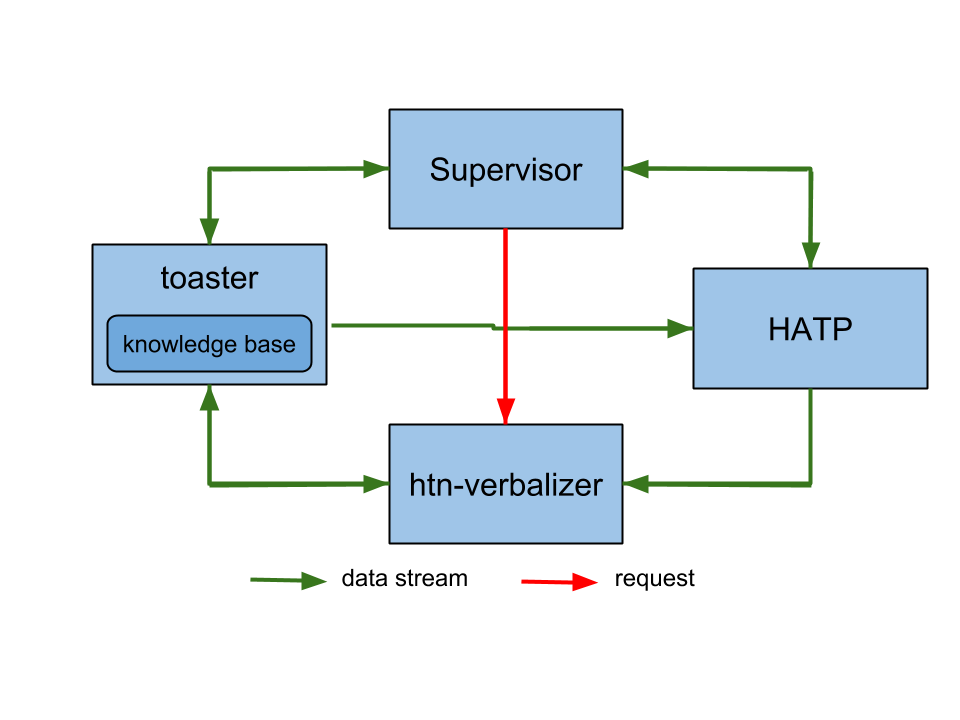
\includegraphics[width=0.6\textwidth]{img/archi.png}
 \end{tabular}
 \caption{Architecture}
 \label{fig:architecture}
   \vspace{-6pt}
 \end{figure}

The figure \ref{fig:architecture}
sums up the architecture and interaction between modules.


\subsection{scenario}
To test our system we created a scenario.
This scenario consist in a collaborative task where a human and a robot has to build a stack of three cubes together. 
Each cube of the stack will need to be processed before being stacked.
%mb put place and needed operation in a table?
\begin{itemize}
\item green cube: it will be placed in bottom and will require polishing.
\item red cube
\item blue cube
\end{itemize}
% TODO: present the scenario
We implement in HATP the  domain of the interaction.


\subsection{Results}
\label{results}
We describe here the interesting steps of the interaction. To have a complete description and video, visit our page\footnote{mypage}.

\subsection{Plan verbalization}
When a human arrives in front of the robot, toaster informs the supervisor that a human is in the working area and is looking toward the robot.
The supervision will then send a request to the htn-verbalizer to init the interaction with the human. It will also request a plan to HATP.

The supervisor will then require the htn-verbalizer to verbalize the plan generated from HATP. %\ref{fig:hatpplan}

% Explain how an action is explained only once
In our scenario, a method has to be done several times by the human. Indeed, the cubes need to be cleaned before being actually processed.
As our system is able to dynamically update the human knowledge, the robot will explain it only the first time.

\subsection{Verbalization during execution}
Once the system finished his explanation about the plan, it informs the human that the execution will start.

%TODO
At action blabla, the human did balabla. The robot was monitoring the action blabla and notice that the post conditions of this action aren't reached. A new plan is then requested to HATP.

The robot inform the human of his mistake and lower his practical knowledge on the concerned task.
We show below a part of the verbalization:
%TODO

Then the robot explains the new plan. In this case, he will have only to explain blabla as the other tasks were already explained in the 1st part of the execution.

During the execution of the new plan, the robot will proceed as for the previous execution.

%TODO: End with metrics: time, number of actions verbalized

%TODO: describe here the interaction, mb with a plan and verbalization output would be good.
% Explain at least 1 replan situation and one situation where an action is needed twice but explained only once

% It would be good to have at least some metrics (number of words/ length of interaction/ explanation with/ without knowledge)
% Some feedback from users?

%%%%%%%%%%%%%%%%%%%%%%%%%%%%%%%%%%%%%%%%%%%%%%%%%%%%%%%%%%%%%%%%%%%%%

%Is this needed? Or in conclusion?
\section{Discussion and perspective on future work}


future work:
In a future paper we would like to conduct a user study enlightening the necessity of  plan verbalization and execution segmentation according to the number of actions to verbalize for each agent to ensure scalability of our solution.
We would like also the user to be able to make requests on actions repartition, leading to a plan negociation before the execution.
In the current study, we consider that the robot knows all the methods and there decomposition. A way to improve this would be to teach the decompositions of tasks to the robot as in\cite{Mohseni2015}.
%In \cite{Mohseni2015}, the system is able to learn task decomposition from naïve user teaching. They also produce suggestion from object physical property and preconditions and postconditions comparison. This provide an easy way to teach an HTN to a system.
To improve the interactivity, we should make possible for the human to request explanations on the robot actions as done in\cite{Lomas2012}.
%Explaining robot actions \cite{Lomas2012}
%https://www.researchgate.net/publication/254007903_Explaining_robot_actions

%human explaining his choice
%Telling more than we can know: Verbal reports on mental processes
%http://people.virginia.edu/~tdw/nisbett&wilson.pdf


\section{Conclusion}
In this paper we show how we were able to explain a plan to a human partner through verbalization.
Our approach is based on a dynamical tracking of the partner's knowledge state, which allows to 
fasten the explanation and to avoid repetitions, thus avoiding the robot to be perceived as "annoying" and reducing the time needed to achieve the task.
This tracking of knowledge also gives the possibility for the robot to choose a plan according to a policy of teaching or efficienty. Finally it also
gives the possibility for the robot to monitor human on higher lever of actions, giving more flexibility for the human to choose the way to perform a task when he has sufficient knowledge.


% ---- Bibliography ----
%
\bibliographystyle{splncs03}
\bibliography{planning.bib,intention.bib,hrteams}

\end{document}
